The general equation of second degree is given by
\begin{align}
ax^2+2bxy+cy^2+2dx+2ey+f=0 \label{eq:solutions/41/ex/gen_quad_eqn}
\end{align}
and can be expressed as
\begin{align}
\vec{x}^T\vec{V}\vec{x}+2\vec{u}^T\vec{x}+f=0 \label{eq:solutions/41/ex/conic_quad_eqn}
\end{align}
where
\begin{align}
\vec{V} &= \vec{V}^T = \myvec{a & b \\ b & c}
\\
\vec{u}^T &= \myvec{d & e}
\end{align}

Comparing \eqref{eq:solutions/41/ex/given_curve_eq} with \eqref{eq:solutions/41/ex/gen_quad_eqn}, we get
\begin{align}
\vec{V} &= \myvec{35  & -6 \\ -6 & 30}
\\
\vec{u}^T &= \myvec{16 & -54}
\end{align}
If $\abs{\vec{V}} > 0$, then \eqref{eq:solutions/41/ex/conic_quad_eqn} is an ellipse. 
\begin{align}
\abs{V} = 
\mydet{
35  & -6 \\ -6 & 30
}
= 1014 > 0
\end{align}
%
\eqref{eq:solutions/41/ex/conic_quad_eqn} can be expressed as
\begin{align}
\label{eq:solutions/41/ex/conic_simp_temp_nonparab_eq}
\vec{y}^T\vec{D}\vec{y} &=  \vec{u}^T\vec{V}^{-1}\vec{u} -f  &  \abs{V} &\ne 0
\\
\vec{y}^T\vec{D}\vec{y} &=  -\eta\myvec{1 & 0}\vec{y}   & \abs{V} &= 0
\label{eq:solutions/41/ex/conic_simp_temp_parab_eq}
\end{align}
with center as 
\begin{align}
    \vec{c} &= - \vec{V}^{-1}\vec{u} & \abs{V} &\ne 0
\end{align}
Calculating the center for given curve we get,
\begin{align}
    \vec{c} &= - \frac{1}{\abs{35*30 - 6*6}}\myvec{30  & 6 \\ 6 & 35}\myvec{16 \\ -54} \\
    &= \frac{1}{1014}\myvec{156 \\ -1794} \\
    &= \myvec{\frac{2}{13}  \\\frac{-23}{13}}
\end{align}

For 
\begin{align} 
\abs{\vec{V}} > 0, \quad \text{or, } \lambda_1 > 0, \lambda_2 > 0 
\end{align} 
\eqref{eq:solutions/41/ex/conic_simp_temp_nonparab_eq} becomes 
\begin{align} \lambda_1y_1^2 +\lambda_2y_1^2 = 
\vec{u}^T\vec{V}^{-1}\vec{u} -f 
\end{align} 
which is the equation of an ellipse with major and minor axes 
parameters
\begin{align} 
\sqrt{\frac{\lambda_1}{\vec{u}^T\vec{V}^{-1}\vec{u} -f}}, 
\sqrt{\frac{\lambda_2}{\vec{u}^T\vec{V}^{-1}\vec{u} -f}} \label{eq:solutions/41/ex/axes_eq}
\end{align}
The characteristic equation of $\vec{V}$ is obtained by evaluating the determinant
\begin{align}
\mydet{\lambda \vec{I}-\vec{V}} = \mydet{\lambda -35 & 6 \\ 6 & \lambda -30} &= 0
\\
\implies \lambda^2 - 65\lambda + 1014 &= 0
\label{eq:solutions/41/ex/ellipse_char_eq}
\end{align}
The eigenvalues are the roots of \eqref{eq:solutions/41/ex/ellipse_char_eq} given by
\begin{align}
\lambda_1 = 39, \lambda_2 = 26
\end{align}


Calculating the major and minor axes lengths using \eqref{eq:solutions/41/ex/axes_eq}, we get
\begin{align}
\vec{u}^T\vec{V}^{-1}\vec{u} &= \nonumber \\
&= \myvec{16 -54}\frac{1}{1014}\myvec{30 & 6 \\ 6 & 35 }\myvec{16 \\ -54} \nonumber \\
&= \frac{1}{1014}\myvec{16 & -54}\myvec{156 \\ -1794} \nonumber \\
&= 98 \nonumber \\
\vec{u}^T\vec{V}^{-1}\vec{u} -f &= 98 - 59 = 39 \\
\sqrt{\frac{\vec{u}^T\vec{V}^{-1}\vec{u} -f}{\lambda_1}} &= \sqrt{\frac{39}{39}} = 1 \\
\sqrt{\frac{\vec{u}^T\vec{V}^{-1}\vec{u} -f}{\lambda_2}} &= \sqrt{\frac{39}{26}} = \frac{\sqrt{6}}{2}
\end{align}


\begin{figure}[!ht]
\centering
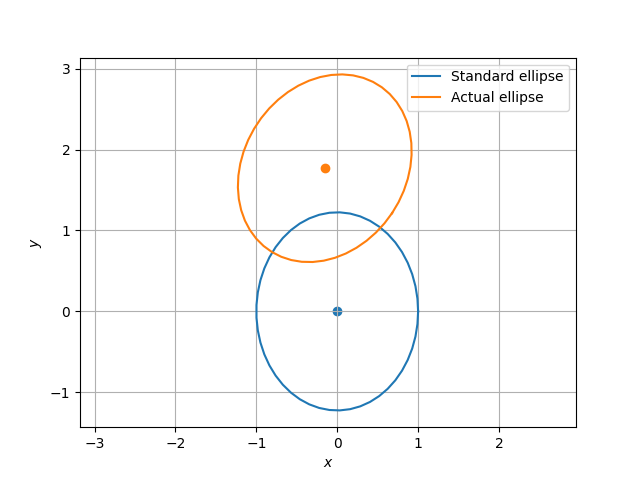
\includegraphics[width=\columnwidth]{./solutions/41/ex/Assignment7.png}

\caption{Ellipse with center \myvec{\frac{2}{13} & \frac{-23}{13}} and having the axes lengths as 1 and $\frac{\sqrt{6}}{2}$}
\label{eq:solutions/41/ex/Fig:Circle}
\end{figure}

